\documentclass[a4paper, 12pt]{article}

\usepackage[utf8]{inputenc}
\usepackage[T1]{fontenc}
\usepackage{geometry}
\usepackage[onehalfspacing]{setspace}
\usepackage[ngerman]{babel} 
\usepackage{csquotes}
\usepackage[backend=biber, style=alphabetic, citestyle=alphabetic-verb]{biblatex}
\usepackage{graphicx}
\usepackage{helvet}
\usepackage[eulergreek]{sansmath}
\usepackage[parfill]{parskip}
\usepackage{enumitem} 
\usepackage{changepage}
\usepackage{listings}
\usepackage{color}
\usepackage[nottoc]{tocbibind}
\usepackage{float}
\usepackage{chngcntr}
\usepackage[titles]{tocloft}
\usepackage{hyperref}
\usepackage{enumitem}
\usepackage[expansion, final]{microtype}
\usepackage{titlesec}
\usepackage{multirow}
\usepackage{graphicx}
\usepackage[labelfont={footnotesize, bf}, textfont={footnotesize, bf}]{caption}
\usepackage[labelfont={footnotesize}, textfont={footnotesize}]{subcaption}
\usepackage{rotating}
\usepackage[table, xcolor=dvipsnames]{xcolor}
\usepackage{fancyhdr}
\usepackage{lastpage} 
\usepackage{amsmath}
\usepackage{pgfplots}
\usepackage{enumitem}
\usepackage{hhline}
\usepackage{colortbl}
\usepackage{booktabs}

\captionsetup[figure]{% use subfigure to confine changes to subcaptions
  justification = RaggedRight, 
  format=hang}

\pgfplotsset{
  tick label style = {font=\sansmath\sffamily},
  every axis label = {font=\sansmath\sffamily},
  legend style = {font=\sansmath\sffamily},
  label style = {font=\sansmath\sffamily},
  compat=1.15
}

\definecolor{standardblue}{RGB}{91,155,213}
\definecolor{darkblue}{RGB}{47,86,122}
\definecolor{standardred}{RGB}{214,92,92}
\definecolor{darkred}{RGB}{132,58,58}

%configuration of figure numbering and table of figures
\counterwithin{figure}{section}
\setlength{\cftfigindent}{0pt}
\newlength{\figlen}

\renewcommand{\cftfigpresnum}{\figurename\enspace}
\settowidth{\figlen}{\cftfigpresnum\cftfigaftersnum}
\addtolength{\cftfignumwidth}{2\figlen}

%configuration of table numbering and table of tables
\counterwithin{table}{section}
\setlength{\cfttabindent}{0pt}

\renewcommand{\cfttabpresnum}{\tablename\enspace}
\settowidth{\figlen}{\cfttabpresnum\cfttabaftersnum}
\addtolength{\cfttabnumwidth}{2.3\figlen}

% make paragraph to fourth section
\titleformat{\paragraph}[hang]{\normalfont\normalsize\bfseries}{\theparagraph}{0em}{}
\titlespacing*{\paragraph}{0pt}{3.25ex plus 1ex minus .2ex}{0.5em}

\setcounter{biburllcpenalty}{9000}
\setcounter{biburlucpenalty}{9000}

\geometry{a4paper, left=25mm, right=15mm, top=25mm, bottom=15mm}

%configure font%
\renewcommand{\familydefault}{\sfdefault}

%configure header%
\geometry{headheight=16pt}
\pagestyle{fancy}
\fancypagestyle{default}{
	\fancyhf{}
	\fancyhead[L]{\nouppercase{\leftmark}}
	\fancyhead[R]{Seite \thepage{} von \pageref{page:last}}
}

\fancypagestyle{table}{
	\fancyhf{}
	\fancyhead[L]{\nouppercase{Verzeichnisse}}
	\fancyhead[R]{Seite \thepage{} von \pageref{page:last}}
}

\fancypagestyle{toc}{
	\fancyhf{}
	\fancyhead[L]{\nouppercase{Inhaltsverzeichnis}}
}

\fancypagestyle{self}{
	\fancyhf{}
	\fancyhead[L]{\nouppercase{Selbstständigkeitserklärung}}
}

\fancypagestyle{tof}{
	\fancyhf{}
	\fancyhead[L]{\nouppercase{Abbildungsverzeichnis}}
	\fancyhead[R]{II}
}

\pagestyle{default}

\interfootnotelinepenalty=10000

%configuration of references%
\bibliography{bibliography}
\DeclareBibliographyCategory{cited}
\AtEveryCitekey{\addtocategory{cited}{\thefield{entrykey}}}

\defbibenvironment{notcited}
  {\list
     {}
     {\setlength{\leftmargin}{0pt}%
      \setlength{\itemindent}{-\leftmargin}%
      \setlength{\itemsep}{\bibitemsep}%
      \setlength{\parsep}{\bibparsep}}}
  {\endlist}
  {\item}


%configure listing%
\renewcommand\lstlistingname{Quelltext}
\renewcommand{\lstlistlistingname}{Quelltextverzeichnis}

\AtBeginDocument{
  \counterwithin{lstlisting}{section}%
}

\makeatletter
\renewcommand{\l@lstlisting}[2]{%
  \@dottedtocline{1}{0em}{4,5em}{\lstlistingname\ #1}{#2}%
}
\makeatother
 

%configure equations
\newcommand{\listequationsname}{Gleichungsverzeichnis}
\newlistof{equations}{loe}{\listequationsname}
\newcommand{\equations}[1]{%
	\addcontentsline{loe}{equations}{\protect Gleichung \numberline{\theequation}#1}\par}

\makeatletter
     \renewcommand*\l@equations{\@dottedtocline{1}{0em}{4em}}
\makeatother

\renewcommand{\cftafterloetitle}{\parindent}

\counterwithin{equation}{section}

% Adjust spacing of equations
\makeatletter
\g@addto@macro\normalsize{%
  \setlength\abovedisplayskip{-5pt}
  \setlength\belowdisplayskip{0pt}
  \setlength\abovedisplayshortskip{-5pt}
  \setlength\belowdisplayshortskip{0pt}
}
\makeatother

%configure appendix%
\newcommand{\listappendicesname}{Anhangsverzeichnis}
\newlistof{appendices}{loa}{\listappendicesname}
\newcommand{\appendices}[1]{\newpage\subsection{#1}
	\refstepcounter{appendices}%
  \addcontentsline{loa}{appendices}
    {\protect Anhang \numberline{\theappendices} #1}\par%
}
\renewcommand{\theappendices}{\Alph{appendices}}

\makeatletter
\newcounter{savesection}
\newcounter{apdxsection}
\renewcommand\appendix{\par
  \setcounter{savesection}{\value{section}}%
  \setcounter{section}{\value{apdxsection}}%
  \setcounter{subsection}{0}%
  \gdef\thesection{\@Alph\c@section}}
\newcommand\unappendix{\par
  \setcounter{apdxsection}{\value{section}}%
  \setcounter{section}{\value{savesection}}%
  \setcounter{subsection}{0}%
  \gdef\thesection{\@arabic\c@section}}
\makeatother

% exclude fields from bibliography
\AtEveryBibitem{%
    \ifentrytype{online}{
        \clearfield{pages}%
        \clearfield{doi}%
        \clearfield{issn}%
        \clearfield{eprint}%
        \clearfield{volume}%
        \clearfield{note}%
        \clearfield{archivePrefix}%%
    }{}
}

% style fields in bibliography
\DeclareFieldFormat[misc]{title}{\glqq#1\grqq}
\DeclareFieldFormat[misc]{date}{(#1)}

\renewcommand{\cftafterloatitle}{\parindent}
\newcommand{\tabitem}{~~\llap{\textbullet}~~}

\title{Fashion Feature Annotation}
\date{\today}
\author{Jerome Wuerf und Eric Mäuer}

%-------------------------------------------------------------------------------

\begin{document}

\makeatletter
\begin{titlepage}
\centering	

\vspace*{2cm}
Universität Leipzig\\
Fakultät für Mathematik und Informatik\\
Institut für Informatik\\
Abteilung Datenbanken

\vspace*{2cm}
{\Large\bfseries \@title \par}

\vspace*{3cm}
Konzeptioneller Programmentwurf\\
für das Big Data Praktikum \\
in der Studienrichtung M. Sc. Data Science

\flushleft
\vspace*{3cm}

\begin{tabular}{p{4cm} p{7cm}}
Eingereicht von: & \@author\\
& Studiengang M. Sc. Data Science
\end{tabular}

\vspace*{1cm}
\begin{tabular}{p{4cm} p{6cm}}
Betreuer: & Moritz Wilke\\
& ScaDS Leipzig
\end{tabular}

\vfill
\@date, Leipzig
\end{titlepage}
\makeatother

\newpage

\pagestyle{toc}

\setcounter{page}{2}

%\tableofcontents
%\newpage
%\setcounter{page}{1}


%\newpage
\pagestyle{default}

\section{Einleitung} \label{sec:intro}
\section{Datensatz} \label{sec:data_set}

Der folgende Abschnitt soll sich mit dem verwendeten Datensatz auseinandersetzen. Dazu gehört eine Evaluation verschiedener Datensätze und die Selektion des am besten geeigneten. Des Weiteren soll auf einige Methoden eingegangen werden, die den gewählten Datensatz auf den hier vorliegenden Anwendungsfall anpassen.

Für die Erstellung eines Datensatzes existieren grundsätzlich zwei Möglichkeiten. Der erste Ansatz besteht darin, die Datensammlung selbst durchzuführen und die Daten beispielsweise von der Webseite eines Fashion-Online-Shops zu extrahieren. Diese Methode bietet einen hohen Grad an Flexibilität, ist allerdings sehr aufwendig. Die Alternative besteht darin einen bereits existierenden Datensatz zu verwenden und die Erstellung so deutlich zu vereinfachen. Aufgrund des großen zeitlichen Aufwands der ersten Variante und der Verfügbarkeit verschiedener vorgefertigter Fashion-Datensätze soll in diesem Projekt der zweite Ansatz verfolgt werden.

Dementsprechend muss aus den verfügbaren Optionen die ausgewählt werden, die den Anforderungen des Projektes am meisten genügt. Mögliche Datensätze sind Fashion Product Images Dataset \cite{FashionProduct2019}, Fashionpedia \cite{Fashionpedia2020}, Fashion-MNIST \cite{FashionMNIST2017} und Deepfashion \cite{DeepFashion2016}. Ein Vergleich der Optionen ist in Tabelle \ref{tab:compareSets} dargestellt. 

\begin{table}[H]
\centering
\resizebox{0.95\textwidth}{!}{%
\begin{tabular}{lll}
\toprule
Datensatz & Vorteile & Nachteile \\ 
\midrule
Fashion Product Images  
    & \tabitem mehr als 44.000 Bilder
    & \tabitem Nicht alle Klassen notwendig\\
    & \tabitem Vielzahl an Klassen/ Attributen
    & \tabitem i.d.R Frontalperspektive\\
    & \tabitem Ein Objekt im Zentrum
    & \tabitem Hintergrund immer weiß
    \bigskip\\
Fashionpedia            
    & \tabitem mehr als 48.000 Bilder 
    & \tabitem Mehrere Objekte pro Bild\\
    & \tabitem Vielzahl an Klassen/ Attributen
    & \tabitem Nicht alle Klassen notwendig\\
    & \tabitem Bilder aus verschiedenen Perspektiven
    &  
    \bigskip\\
Fashion-MNIST           
    & \tabitem integriert in Tensorflow-Datasets
    & \tabitem geringe Anzahl an Klassen/ Attributen\\
    & \tabitem mehr als 60.000 Bilder
    & \tabitem Schwarz-Weiß-Bilder
    \bigskip\\
Deepfashion             
    & \tabitem mehr als 800.000 Bilder         
    & \tabitem unterteilt in verschiedene Benchmarks\\ 
    & \tabitem Vielzahl an Klassen/ Attributen
    & \tabitem Benötigte Attribute nicht in allen Benchmarks\\
\bottomrule
\end{tabular}}
\caption{Vergleich verschiedener Fashion-Datensätze}
\label{tab:compareSets}
\end{table}

Aufgrund dessen, dass die Kleidung i. d. R. isoliert abgebildet wird und eine ausreichende Auswahl an Attributen existiert, soll der Fashion Product Images Datensatz verwendet werden. Fashionpedia wurde ausgeschlossen, weil zusätzlich zu der Klassifizierung noch eine Segmentierung des Bildes notwendig wäre und Fashion-MNIST aufgrund dessen, dass dieser keine befriedigende Komplexität für diesen Anwendungsfall bietet. Die Daten des In-shop Clothes Retrieval Benchmark aus Deepfashion stellen ebenfalls einen geeigneten Datensatz dar, sollen jedoch vorerst nicht verwendet werden. Allerdings soll die Möglichkeit offen gehalten werden diesen in Teilen oder komplett zusätzlich zu nutzen, um eventuelle Ungleichverteilungen auszugleichen oder die Datenmenge zu vergrößern.

Bevor der Datensatz verwendet werden kann, müssen jedoch noch einige Analysen durchgeführt werden und infolgedessen Anpassungen vorgenommen werden. Zu den Änderungen gehört die Selektion relevanter Merkmale (Accessoires werden beispielsweise nicht berücksichtigt) sowie eine sinnvolle Zusammenfassung einiger Werte (z. B. werden Jeans und Leggings Hosen zugeordnet). In Abbildung \ref{fig:evaluation} sind die Verteilungen und möglichen Ausprägungen der gewählten Klassen dargestellt.

\begin{figure}[H]
    \centering
    \begin{subfigure}[c]{0.32\linewidth}
        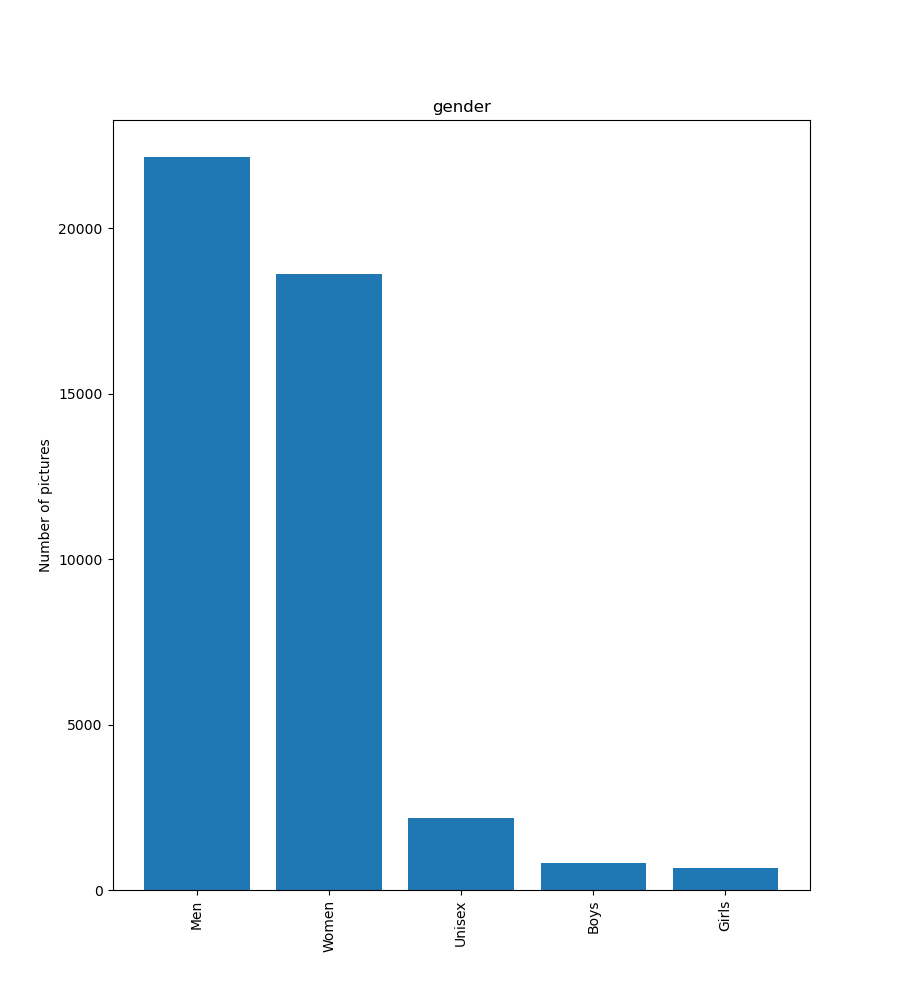
\includegraphics[width=\linewidth]{Ausarbeitung/images/gender.png}
    \end{subfigure}
    \begin{subfigure}[c]{0.32\linewidth}
        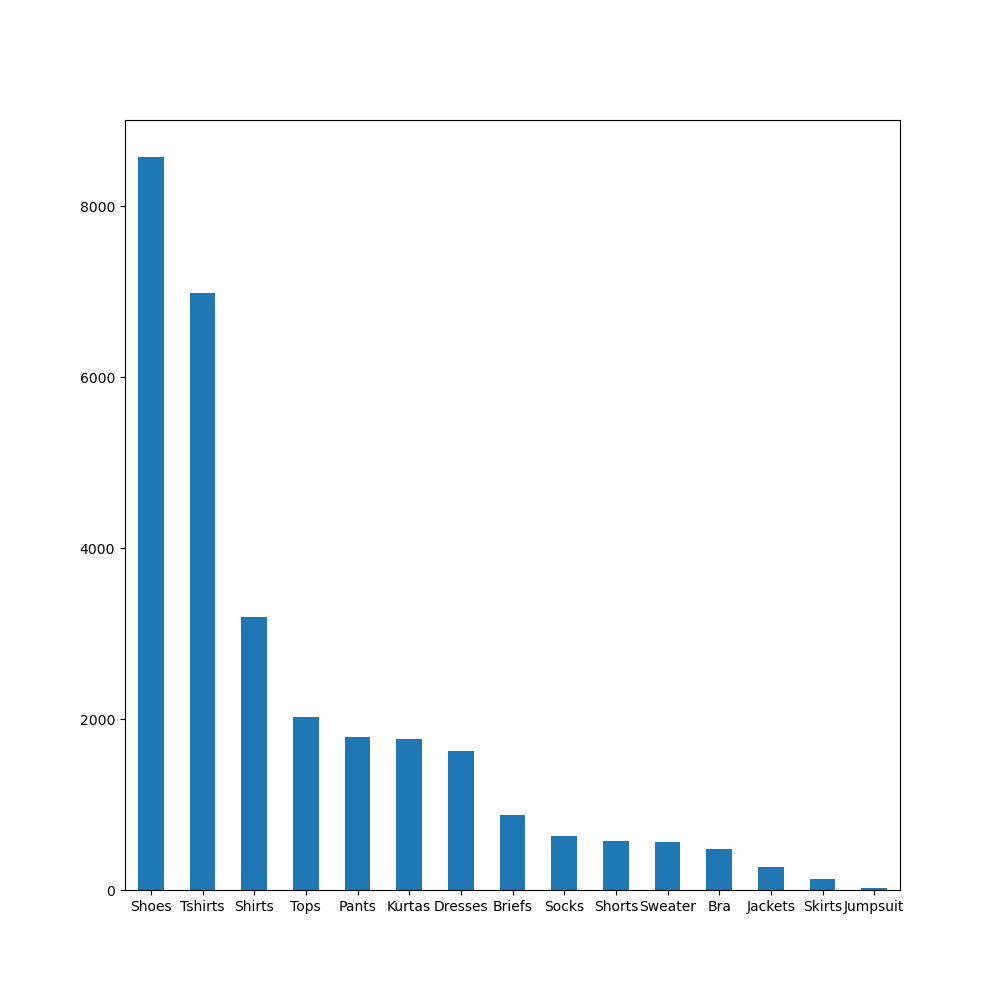
\includegraphics[width=\linewidth]{Ausarbeitung/images/articleType.png}
    \end{subfigure}
    \begin{subfigure}[c]{0.32\linewidth}
        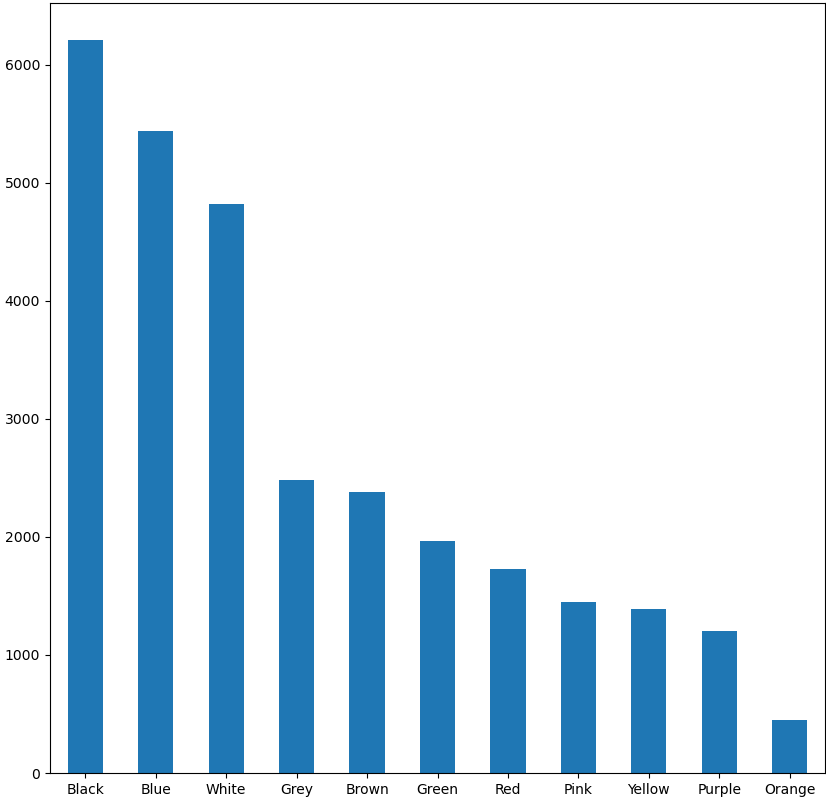
\includegraphics[width=\linewidth]{Ausarbeitung/images/baseColour.png}
    \end{subfigure}
    \caption{Verteilungen der ausgewählten Merkmale}
    \label{fig:evaluation}
\end{figure}

Für die Erstellung des verwendeten Datensatzes werden die Bilder normalisiert und augmentiert. Das heißt, sie werden auf eine einheitliche Größe gebracht und die Farbwerte auf ein Intervall von null bis eins skaliert. Bei der Erweiterung der Bilder sollen z. B. die Rotation, Helligkeit und die Spiegelung zufällig verändert werden.

Die Labels werden in Form eines Multi-Hot codierten Vektors repräsentiert. Dementsprechend steht jede eins dafür, dass eine bestimmte Ausprägung in dem Bild vorkommt. In Abbildung \ref{fig:multihot} ist das Prinzip vereinfacht dargestellt. Diese Form der Darstellung wird benötigt, damit das Modell eine Multi-Label-Klassifizierung durchführen kann.

\begin{figure}[H]
    \centering
    
\includegraphics[width=0.3\linewidth]{Ausarbeitung/images/MultiHotEncoding.png}
    \caption{Multi-Hot-Kodierung eine blauen T-Shirts für Männer}
    \label{fig:multihot}
\end{figure}

Der Datensatz soll in Traings-, Test- und Validierungsdaten aufgeteilt werden. Dabei sollen 80\% der Daten als Trainingsdaten dienen und der Rest wird gleichmäßig auf die anderen beiden Teile aufgespalten.
\section{Modell} \label{sec:model}

Nachdem erfolgreich ein Datensatz erzeugt wurde, kann auf diesem mithilfe von maschinellem Lernen ein Modell angelegt werden, das letztendlich die Klassifizierung durchführen soll. Im Folgenden soll näher auf die angewendete Architektur und die Besonderheiten bei der Verwendung dieser eingegangen werden.

Als Modell soll ein "artificial neural network" (ANN) verwendet werden, das mithilfe eines überwachten Lernverfahrens trainiert wird. ANNs besitzen den Vorteil, dass sie sehr gut mit großen Datenmengen umgehen können und nicht auf eine Gleichverteilung der Daten angewiesen sind. Zudem generalisieren sie Problem, sodass auch unbekannte Eingaben verarbeitetet werden können. Ein weiterer bedeutender Vorteil von ANNs ist, dass sie sich sehr gut für die Verarbeitung von Bilddaten eignen. \cite{Mahanta2020}

Die aktuell beste Architektur für die Klassifizierung von Bildern stellen Convolutional Neuronal Networks (CNN) dar. Diese setzen sich grundsätzlich aus zwei Teilen zusammen. Der erste Teil dient zur Merkmalsextraktion und der zweite zur Klassifikation. Nach diesem Prinzip werden zuerst Merkmale, wie Kanten, im gesamten Bild gefunden und anschließend anhand ihrer Komposition klassifiziert. Vertiefende Informationen zu CNNs können unter anderem in \cite{Goodfellow2016} oder in \cite{CS2020} nachgelesen werden.

Im Bezug auf dieses Projekt gibt es noch Anpassungen, die für die Erfüllung der Zielsetzung beachtet werden müssen. Die erste Besonderheit besteht darin, dass Transfer Learning genutzt werden soll. Durch die Verwendung eines vortrainierten CNNs verringert sich die Anzahl der zu lernenden Parameter und die damit verbundene Trainingszeit deutlich. Während des Trainings werden somit nur Gewichte der Klassifikationsschichten gelernt. Optional können auch die Parameter der letzten Schichten des vortrainierten CNNs weiter angepasst werden, um dessen Merkmalsextraktion datensatzspezifischer zu gestalten.

Die zweite Anpassung ist notwendig, um eine Multi-Label-Klassifikation durchführen zu können. Dazu wird eine Aktivierungsfunktion benötigt, die im Gegensatz zu Softmax, jede Aktivierung unabhängig von den anderen berechnet. Diese Unabhängigkeit der Ergebnisse ist notwendig, da ein Objekt mehreren verschiedenen Klassen zugeordnet werden soll. Eine Aktivierungsfunktion, die diese Anforderung erfüllt ist beispielsweise Sigmoid. Vorerst soll dann aus jeder Kategorie die maximale Aktivierung als Ergebnis verwendet werden. Für Farben wäre eine spätere Ergänzung denkbar, die es ermöglicht, mehrere Werte zu erkennen, indem alle Aktivierungen über einen bestimmten Schwellenwert gewählt werden. 

Abschließend werden alle bisher beschriebenen Komponenten in eine Architekturübersicht zusammengefasst \ref{fig:generalArch}. Zuerst werden die Rohbilder durch Augmentation in ihrer Stückzahl erweitert, skaliert und normalisiert. Im Anschluss werden die Bilder durch das vortrainierte CNN zu einen merkmalsangereicherten Volumen transformiert. Dieses Volumen wird dann in ein eindimensionales Array abgeflacht, welches den Input zu mehreren aufeinanderfolgenden Klassifikationsschichten bildet. Die Klassifikationsschichten sind vollvernetzt. Letztlich verarbeitet die Sigmoidfunktion den Output der Klassifikation zu den maximalen Aktivierungen.
\begin{figure}[H]
	\centering
	
\includegraphics[width=0.9\linewidth]{images/general_architecture.png}
	\caption{Architekturübersicht}
	\label{fig:generalArch}
\end{figure}


\section{Schlussteil} \label{sec:conclusion}

In den beiden vorherigen Abschnitten wurde erläutert, wie die Zielsetzung des Projektes erfüllt werden soll. Dabei wurde der \say{Fashion Product Images} Datensatz als Grundlage für das Training gewählt. Es wurden die Kategorien vorgestellt, denen eine Objekt zugeordnet werden kann und wie diese verteilt sind. Die Multi-Label-Klassifizierung soll mithilfe eines CNNs durchgeführt werden, das durch Transfer Learning trainierte Schichten verwendet. 

Für eine Evaluierung der Ergebnisse sollen stets Metriken wie Precision und Recall ermittelt werden, um die günstigste Lösungsstrategie zu finden. Infolgedessen kann es im Laufe des Entwicklungsprozesses noch zu Änderungen oder Erweiterungen kommen, die von diesem Konzept abweichen.

\pagestyle{table}

\section*{Literaturverzeichnis}
\printbibliography[heading=none, category=cited]
\label{page:last}
\end{document}